\documentclass[main.tex]{subfiles}
\begin{document}
在\S\ref{I.2 pratical_thermodynamics}中已经提到,要确定混合物体系的完整热力学性质,除它的某一可逆过程热容关于体系状态的完整函数外,还需要知道其$pVTn_i$状态方程。这样,就能过依照偏摩尔量的测量原理,把确定各组份化学势所需的偏摩尔响应函数都获知,以便确定体系最基本的热力学函数——内能和熵——的微分表达式。

但是,样的实验工作量会随组份数的增多而成倍增加。我们朴素地希望,能否仅测量各组份纯物质的性质$M_i^*\left(X,Y\right)$,就能通过形如
\[M\left(X,Y,\left\{n_i\right\}\right)=\sum_i n_i M_i^*\left(X,Y\right)\]
而得到混合物同样条件下任一组成$\left\{n_i\right\}$的性质$M\left(X,Y,\left\{n_i\right\}\right)$了呢?很遗憾,这种针对纯物质性质的加和性,并不普遍成立。普适的加和性只有偏摩尔量的加和性(式\eqref{eq:II.2_additivity_partial_molar_quantity_1}或\eqref{eq:II.2_additivity_partial_molar_quantity_2})。回忆《物理化学》的知识,道尔顿分压定律,好像就是形如上式的某种针对纯物质的加和性。是否能够根据理想气体混合物满足道尔顿分压定律的性质,来得出理想气体混合物的各热力学性质满足针对其纯物质性质的加和性呢?本节将讨论这个问题,并最终确定理想气体混合物的完整定义。

我们知道\footnote{见《物理化学》\S1.1之“气体分子运动公式对几个经验定律的说明”。},理想气体除了在单组份的情况下满足
\begin{enumerate}
    \item 玻意耳定律:$pV=\text{温度的函数}$;
    \item 焦耳定律:内能是温度的函数\footnote{亦可见《物理化学》\S 2.8式(2.18)。};
    \item 阿伏伽德罗定律:同温同压下,一摩尔各种气体的体积相等;
\end{enumerate}
这三条之外,在多组份的情况下还要满足道尔顿分压定律。而后者说的就是多组份气体混合物压强的一种加和性:混合气体的压强等于各组份气体同温同体积下的压强之和,写成式子就是
\[p\left(T,V\right)=\sum_i p^*_i\left(T,V\right)\]
其中$p_i^*\left(T,V\right)$是组份$i$纯物质的压强。如果这些组份的纯物质气态都是理想气体,则有$p_i^*\left(T,V\right)=n_iRT/V$,由道尔顿分压定律可得$p=\sum_in_iRT/V=nRT/V$,即混合后的体系将仍是一个理想气体。

这四条定律,似乎给出了一个气体混合物的$pVTn_i$状态方程,即$V\left(T,p,\left\{n_i\right\}\right)=RT\sum_in_i/p$。尽管还缺少热容,但至少应该足以预测体系在任一等温实验下的性质了。以下这个实例说明,仅从上列四条定律,也不足以预测气体混合物在等温实验的热力学行为。

考虑如图\ref{fig:gas_mixture_experiment}所示的实验。整个体系与环境保持温度为$T$。达到平衡时,左侧硬壁缸内的混合气体压强为$p$,右侧为一系列品质相同的气球,经过半透膜的分隔,它们各只含有纯气体$i$,气球膨胀的大小可反映气球内的压强大小$p^*_i$(示意图中显得一样大了)。$p^*_i$各是多少一般将取决于左侧混合气体的组成$\left\{x_i\right\}$ 。

仅靠道尔顿分压定律和基本热力学关系,是无法给出右侧各气球的压强$p^*_i$应是多少的。还需要规定,理想气体混合物在这样的实验中:给定温度$T$的平衡态下,任一能通过半透膜的组份$i$,在膜两边的分压相等。写成式子就是:
\begin{equation}
    \label{eq:II.3_ideal_gas_mixture_partial_pressure_rule}
    p^*_i\left(T\right)=x_ip\left(T\right),\quad\text{理想气体混合物}
\end{equation}

\begin{figure}[ht]
    \centering
    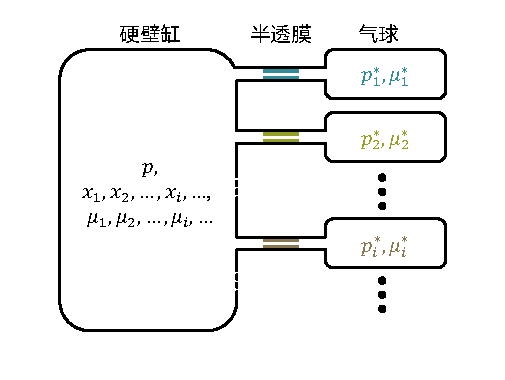
\includegraphics{../images/gas_mixture_experiment.pdf}
    \caption{确定气体混合物行为的实验示意图。整个体系与环境保持温度为$T$。达到平衡时左侧硬壁缸内的混合气体压强为$p$,右侧为一系列同品质的气球,经半透膜,它们只含有纯气体$i$,气球膨胀的大小可反映气球内的压强大小$p^*_i$(示意图中显得一样大了)。$p^*_i$各是多少一般将取决于左侧混合气体的组成$x_1,x_2,\cdots,x_i,\cdots$,但具体取决方式依赖气体混合物的状态方程。理想气体混合物满足$p^*_i=x_ip$。}
    \label{fig:gas_mixture_experiment}
\end{figure}

由于膜右室是单组份理想气体,由$\mu_i^*=\mu_i^*\left(T,p\right)$以及恒温过程$\mathrm{d}T=0$,
\begin{align*}
    \mathrm{d}\mu_i^* & =\left.\frac{\partial\mu_i^*}{\partial p}\right|_{T}\mathrm{d}p \\
                      & =V_i^*\left(T,p\right)\mathrm{d}p                               \\
                      & =\frac{RT}{p}\mathrm{d}p=RT\mathrm{d}\ln p
\end{align*}
因此由相平衡条件$\mu_i=\mu_i^*$和理想气体混合物的规定(式\eqref{eq:II.3_ideal_gas_mixture_partial_pressure_rule}),
\[\mathrm{d}\mu_i=\mathrm{d}\mu_i^*=RT\mathrm{d}\ln p_i^*=RT\mathrm{d}\ln\left(x_ip\right)\]
以上对所有组份$i$均成立。可见,体系这一特定实验中的性质规定,其实是规定了理想气体混合物的偏摩尔吉布斯自由能的表达形式。因此,我们为理想气体混合物写下如下定义性质的化学势表达式:恒定$T$下,理想气体混合物的任意组成$i$的化学势均满足
\begin{equation}\label{eq:II.3_def_ideal_gas_mixture_mu}
    \mathrm{d}\mu_i^\text{ig}\left(T,p,\left\{n_j\right\}\right)=RT\mathrm{d}\ln\left(x_i p\right)
\end{equation}
其中上标“ig”表示理想气体。

我们分析一下这个式子蕴含的意义。作为一个状态函数,组份$i$在理想气体混合物中的化学势$\mu_i^\text{ig}$自然应是状态参量$\left(T,p,\left\{n_i\right\}\right)$的函数。它在恒定$T$($\mathrm{d}T=0$)下的微分式理应形如
\[\mathrm{d}\mu_i^\text{ig}\left(T,p,\left\{n_j\right\}\right)=\left.\frac{\partial \mu_i^\text{ig}}{\partial p}\right|_{T,\left\{n_j\right\}}\mathrm{d}p+\sum_j\left.\frac{\partial\mu_i^\text{ig}}{\partial n_j}\right|_{T,p,\left\{n_{k\neq j}\right\}}\mathrm{d}n_j\]
而式\eqref{eq:II.3_def_ideal_gas_mixture_mu}等号右边的微分式$\mathrm{d}\ln\left(x_ip\right)$可推算至以下形式
\[\mathrm{d}\ln\left(x_ip\right)=\mathrm{d}\ln p+\mathrm{d}\ln n_i\]
其中用到了$x_i=n_i/\sum_jn_j$以及体系总摩尔数恒定(封闭系统)$\mathrm{d}n=\sum_i\mathrm{d}n_i=0$。故有
\begin{align*}
    \left.\frac{\partial \mu_i^\text{ig}}{\partial p}\right|_{T,\left\{n_j\right\}}             & =V_i^\text{ig}=RT\mathrm{d}\ln p                                                \\
    \left.\frac{\partial \mu_i^\text{ig}}{\partial n_j}\right|_{T,p,\left\{n_{k\neq j}\right\}} & =\left\{\begin{array}{ll}0,&j\neq i\\RT\mathrm{d}\ln n_i,&j=i\end{array}\right.
\end{align*}

理想气体混合物化学势定义式\eqref{eq:II.3_def_ideal_gas_mixture_mu}是以微分关系的形式给出的。我们之所以不直接用明显的表达式来定义这个模型体系,是因为热力学函数的绝对值是不可知的,只有其变化量是可知的。用微分表达式来规定规律性,可供我们随时通过式\eqref{eq:I.1_integral_of_function}来进行任意状态之间的热力学函数变化量,故有最好的一般性和灵活性。所以我们要习惯用微分关系来定义模型体系的方式。例如,我们可任选某压强$p^\circ$作为参考压强,则理想气体混合物等温等组分的体积变化过程各组份的化学势变化就是
\begin{equation}\label{eq:II.3_ideal_gas_mixture_mu_p0}
    \begin{aligned}
        \mu_i^\text{ig}\left(T,p,\left\{n_j\right\}\right)-\mu_i^\text{ig}\left(T,p^\circ,\left\{n_j\right\}\right) & =\int_{p^\circ}^p\mathrm{d}\mu_i^\text{ig}\left(T,p^\prime,\left\{n_j\right\}\right) \\
                                                                                                                    & =RT\int_{p^\circ}^p\mathrm{d}\ln\left(x_ip^\prime\right)                             \\
                                                                                                                    & =RT\ln\left(\frac{x_ip}{p^\circ}\right)
    \end{aligned}
\end{equation}
《物理化学》书上的理想气体混合物化学势的定义式(\S 4.5式(4.31))只是具体选择$p^\circ=p\stst$作为惯例而已。

总结理想气体混合物一共要遵守的定律就是:气体混合物在任何组成下遵循——
\begin{enumerate}
    \item 玻意耳定律:$pV=\text{温度的函数}$;
    \item 焦耳定律:内能是温度的函数\footnote{亦可见《物理化学》\S 2.8式(2.18)。};
    \item 阿伏伽德罗定律:同温同压下,一摩尔各种气体的体积相等;
    \item 道尔顿分压定律:混合气体的压强等于各组份气体同温同体积下的压强之和。
    \item 给定温度$T$的平衡态下,任一能通过半透膜的组份$i$,在膜两边的分压相等。
\end{enumerate}

式\eqref{eq:II.3_def_ideal_gas_mixture_mu}足以给出理想气体混合物的完整热力学性质,以下列出部分。由式\eqref{eq:I.1_Maxwell_GnT}和式\eqref{eq:I.1_Maxwell_GTp}有,
\begin{align}
    S^\text{ig}_i & =-\left.\frac{\partial \mu^\text{ig}_i\left(T,p,\left\{n_j\right\}\right)}{\partial T}\right|_{p,\left\{n_j\right\}}=S_0-R\left[\ln x_i+\ln \left(p/p^\circ\right)\right] \\
    V^\text{ig}_i & =\left.\frac{\partial\mu^\text{ig}_i\left(T,p,\left\{n_j\right\}\right)}{\partial p}\right|_{T,\left\{n_j\right\}}=\frac{RT}{p}
\end{align}
其中$S_0\equiv-\left(\partial\mu_i^\text{ig}\left(T,p^\circ,\left\{n_j\right\}\right)/\partial T\right)_{\left\{n_i\right\}}$。恒压恒组成下,又由式\eqref{eq:I.1_heat_capacity_entropy_p}和式\eqref{eq:I.1_Maxwell_GTp}有
\begin{align}
    \left.\frac{\partial S^\text{ig}}{\partial T}\right|_{p,\left\{n_i\right\}} & =\frac{C_p}{T} \\
    \left.\frac{\partial S^\text{ig}}{\partial p}\right|_{T,\left\{n_i\right\}} & =-\frac{nR}{p}
\end{align}
故理想气体混合物的熵的完整全微分式是
\[\mathrm{d}S^\text{ig}=\frac{C_p}{T}\mathrm{d}T-\frac{nR}{p}\mathrm{d}p+\sum_i\left[S_0-R\ln x_i-R\ln\left(p/p^\circ\right)\right]\mathrm{d}n_i\]
恒定$T$、$p$下,由偏摩尔量加和性,
\[S^\text{ig}\left(T,p,\left\{n_i\right\}\right)=\sum_in_i\left[S_0-R\ln x_i-R\ln\left(p/ p^\circ\right)\right]\]
故同条件下的混合熵变(即把$n_1,n_2,\cdots$纯物质混合为组成是$\left\{n_i\right\}$的气体混合物的熵变)
\begin{align*}
    \Delta_\text{mix}S^\text{ig} & =S^\text{ig}\left(T,p,\left\{n_i\right\}\right)-\sum_i n_i S^\text{*,ig}\left(T,p\right)                            \\
                                 & =\sum_in_i\left[S_0-R\ln x_i-R\ln\left(p/p^\circ\right)\right]-\sum_in_i\left[S_0-R\ln\left(p/p^\circ\right)\right] \\
                                 & =-R\sum_in_i\ln x_i
\end{align*}
其中利用到纯物质$S_i^{*,\text{ig}}=S_i^\text{ig}\left(T,p,x_i=1\right)$。

然后我们推导一下混合吉布斯自由能变。利用偏摩尔量的加和性,
\begin{align*}
    \Delta_\text{mix}G^\text{ig} & =G^\text{ig}\left(T,p,\left\{n_i\right\}\right)-G^\text{*,ig}\left(T,p\right)                               \\
                                 & =\sum_in_i\left(\mu_i^\text{ig}\left(T,p,\left\{n_j\right\}\right)-\mu_i^\text{*,ig}\left(T,p\right)\right)
\end{align*}
而由式\eqref{eq:II.3_def_ideal_gas_mixture_mu},
\[\mu_i^\text{ig}\left(T,p,\left\{n_j\right\}\right)-\mu_i^\text{*,ig}\left(T,p\right)=RT\int_{1}^{x_i}d\ln\left(x_i^\prime p\right)=RT\ln x_i\]
故有
\[\Delta_\text{mix}G^\text{ig}=RT\sum_in_i\ln x_i=-T\Delta_\text{mix}S^\text{ig}\Rightarrow\Delta_\text{mix}H^\text{ig}=0\]
其中后面的等号和结论是与混合熵变的表达式比较而得。这些都是理想气体混合物的重要的热力学特征。带$\Delta_\text{mix}$的函数变化量叫混合函数这将在\S\ref{sec:II.4 real_mixture}节中混合函数一节详细讨论。按其定义,若一性质的混合函数为零,就说明混合物体系的该性质具有针对其各组份纯物质性质的加和性。这是对本节开头提出的问题的回应。
\end{document}